\documentclass{article}
\usepackage{etex}
\usepackage{amsmath}
\usepackage{pdfpages}
\usepackage{tikz}
\usepackage{subcaption}
\usepackage{pgf-umlsd}
\usepackage{pgfplots}
\usepackage{geometry}
\geometry{
	a4paper,
	left=25.4mm,
	right=25.4mm,
	top=25mm,
	bottom=25.4mm
	}
\begin{document}

\includepdf{title.pdf}

\tableofcontents
\listoffigures

\newpage

\section{Why Paxos?}
Paxos is a consensus algorithm that allows a group of processes to agree on a single value, even in the presence of failures. It is designed to work in asynchronous distributed systems, where processes may fail or messages may be lost. Paxos is widely used in distributed systems for achieving fault tolerance and ensuring consistency.
The algorithm is based on the idea of a "proposer" that suggests a value, "acceptors" that vote on the proposed value, and "learners" that learn the agreed-upon value. The algorithm ensures that even if some processes fail, as long as a majority of processes are functioning, they can still reach consensus.
Paxos is particularly useful in scenarios where a distributed system needs to maintain a consistent state across multiple nodes, such as in databases, distributed file systems, and cloud computing platforms. It provides a robust and reliable way to achieve consensus, making it a popular choice for building fault-tolerant distributed systems.

\section{Java Implementation of the Robust Key-Value Store}

\subsection{Java classes}
For our implementation with Java and the Akka framework, we have created the following classes:

\begin{itemize}
    \item \texttt{Main}: The main class that creates the different actors and configures the system. It is also the class that computes the statistics at the end of the simulation.

    \item \texttt{Process}: The actor class. The obstruction-free consensus algorithm is implemented in this class.

    \item \texttt{AbortMsg}: The class that represents the abort message sent between the processes.

    \item \texttt{AckMsg}: The class that represents the acknowledgment (ACK) message sent between the processes.

    \item \texttt{CrashMsg}: The class that represents the crash message sent between the processes. When a process receives a crash message, it will enter in the fault-prune mode.

    \item \texttt{DecideMsg}: The class that represents the decide message sent between the processes.

    \item \texttt{WriteAck}: The class that represents the write acknowledgments sent between the processes.

    \item \texttt{Pair}: Used to store (est and estballot) the values inside the states map.
    \item \texttt{GatherMsg}: The class that represents the GATHER message sent between the processes.
    
    \item \texttt{ImposeMsg}: The class that represents the IMPOSE message sent between the processes.
    
    \item \texttt{Members}: The class that contains the processes' references.
    
    \item \texttt{Pair}:  The class that represents a pair of values (est and estballot) used in the states map.
    
    \item \texttt{ReadMsg}: The class that represents the read message sent between the processes.
\end{itemize}

We didn't want to use multiple threads in the \texttt{Process} class due to the large number of processes
being launched. It is more efficient to let the Akka framework's logic thread handle the processes.
% Therefore, we implemented a state machine in the \texttt{Process} class to manage the different states
% of the functions: sending the initial read request, waiting for a quorum of responses, sending the
% write request, and finally, waiting for a quorum of write acknowledgments.


\newpage
\subsection{Akka Design}

\begin{figure}[h!]
\centering

\begin{sequencediagram}
    \newthread{main}{main}
    \newinst{a}{Correct Process  A}
    \newinst[1]{b}{Correct Process B}
    \newinst[1]{c}{Failed Process C}

    \mess{main}{refs}{a}
    \mess{main}{refs}{b}
    \mess{main}{refs}{c}
    \mess{main}{crash}{c}
    \mess{main}{launch}{a}
    \mess{main}{launch}{b}
    \begin{sdblock}{write}{B Writes}
        \begin{call}{b}{Read request}{a}{Read response (ts)}
        \end{call}
        \begin{call}{b}{Write request (val, ts)}{a}{Write ack}
        \end{call}
    \end{sdblock}
    \begin{sdblock}{read}{A reads}
        \begin{call}{a}{Read request}{b}{Read response (val, ts)}
        \end{call}
        \begin{call}{a}{Write request (val, ts)}{b}{Write ack}
        \end{call}
    \end{sdblock}
    \mess{a}{done, stats}{main}
    \mess{b}{done, stats}{main}
\end{sequencediagram}

\caption{Sequence diagram of the Akka design}
\end{figure}
\newpage
\subsection{Statistics computation}

TODO

Throughout the simulation, the processes continuously collect data for
the statistics. At the end of the simulation, the main class will compute this data:

% \begin{itemize}
%     \item The time taken for each process to complete a write operation.
%     \item The time taken for each process to complete a read operation.
%     \item The average time spend by a process to complete all the write operations.
%     \item The average time spend by a process to complete all the read operations.
%     \item The throughput of the system.
% \end{itemize}

For the throughput, we have used the formula :
$$
\text{Throughput} = \frac{\text{Number of operations}}{\text{Total time}}
$$

\newpage

\section{Performance analysis}
The simulation has different parameters that can be changed to test the performance of the system. The main parameters are:

\begin{itemize}
    \item $N$ The number of processes and $f$ the number of processes which can fail.
    \item $t_{le}$ The fixed timeout.
    \item $\alpha$ The probability of failure of a process.
\end{itemize}

Since we need a quorum, $f$ must be less than $N/2$. Thus,
we have different scenarios to test the performance of the simulation
with $(N,f) \in \{(3,1),(10,4),(100,49)\}$, $t_{le} \in \{0.5,1,1.5,2\}$ and $\alpha \in \{0,0.1,1\}$.

\subsection{Results for a fixed timeout $t_{le}$}
Let's now analyze the results for a fixed timeout $t_{le}$ and different values of $N$.

\begin{figure}[h!]
    \centering
    \begin{subfigure}{0.55\textwidth}
    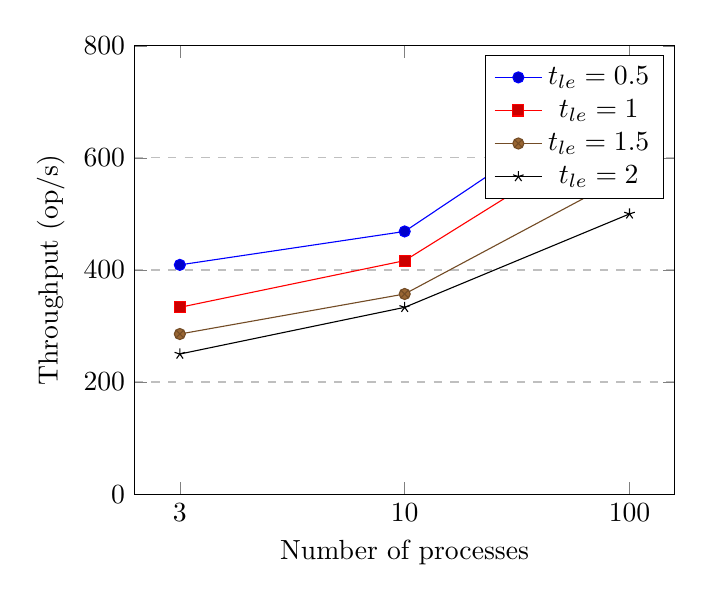
\begin{tikzpicture}
        \begin{axis}[
            xlabel={Number of processes},
            ylabel={Throughput (op/s)},
            xtick=data,
            symbolic x coords={3, 10, 100},
            ymin=0, ymax=800,
            ymajorgrids=true,
            grid style=dashed
        ]
        \addplot coordinates {(3, 409.09) (10, 468.75) (100, 737.10)};
        \addlegendentry{$t_{le} = 0.5$}
        \addplot coordinates {(3, 333.33) (10, 416.67) (100, 666.67)};
        \addlegendentry{$t_{le} = 1$}
        \addplot coordinates {(3, 285.71) (10, 357.14) (100, 571.43)};
        \addlegendentry{$t_{le} = 1.5$}
        \addplot coordinates {(3, 250) (10, 333.33) (100, 500)};
        \addlegendentry{$t_{le} = 2$}
        \end{axis}
    \end{tikzpicture}
    \caption{Throughput comparison }
\end{subfigure}%
\begin{subfigure}{.55\textwidth}
    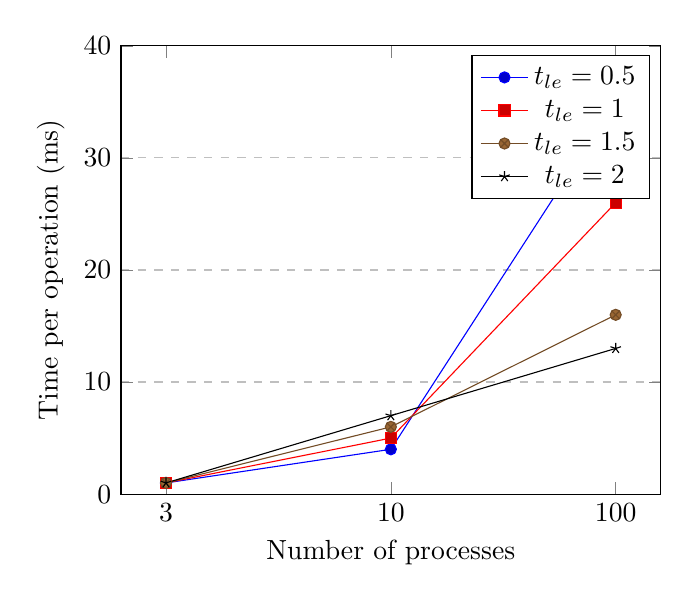
\begin{tikzpicture}
        \begin{axis}[
            xlabel={Number of processes},
            ylabel={Time per operation (ms)},
            xtick=data,
            symbolic x coords={3, 10, 100},
            ymin=0, ymax=40,
            ymajorgrids=true,
            grid style=dashed
        ]
        \addplot coordinates {(3, 1) (10, 4) (100, 35)};
        \addlegendentry{$t_{le} = 0.5$}

        \addplot coordinates {(3, 1) (10, 5) (100, 26)};
        \addlegendentry{$t_{le} = 1$}
        \addplot coordinates {(3, 1) (10, 6) (100, 16)};
        \addlegendentry{$t_{le} = 1.5$}
        \addplot coordinates {(3, 1) (10, 7) (100, 13)};
        \addlegendentry{$t_{le} = 2$}
        \end{axis}
    \end{tikzpicture}
    \caption{Operation execution time comparison}
\end{subfigure}

\caption{Performance analysis for a fix timeout}
\end{figure}

\begin{figure}[ht!]
    \centering
    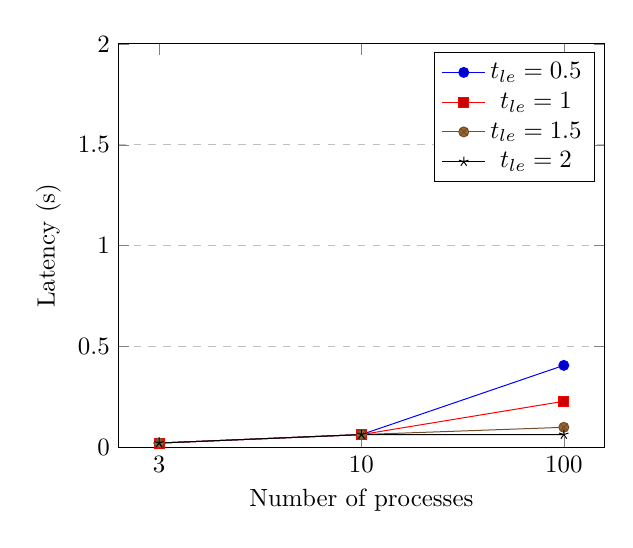
\begin{tikzpicture}[scale=0.9]
        \begin{axis}[
            xlabel={Number of processes},
            ylabel={Latency (s)},
            xtick=data,
            symbolic x coords={3, 10, 100},
            ymin=0, ymax=2,
            ymajorgrids=true,
            grid style=dashed,
        ]
        \addplot coordinates {(3, 0.022) (10, 0.064) (100, 0.407)};
        \addlegendentry{$t_{le} = 0.5$}
        \addplot coordinates {(3, 0.022) (10, 0.064) (100, 0.229)};
        \addlegendentry{$t_{le} = 1$}
        \addplot coordinates {(3, 0.022) (10, 0.064) (100, 0.1)};
        \addlegendentry{$t_{le} = 1.5$}
        \addplot coordinates {(3, 0.022) (10, 0.064) (100, 0.064)};
        \addlegendentry{$t_{le} = 2$}
        \end{axis}
    \end{tikzpicture}
    \caption{Latency comparison for a fix timeout}
\end{figure}


% We can observe that throughput increases with the number of processes. However,
% the growth factor is not linear. Adding a significantly larger number of processes
% does not lead to a substantial increase in throughput, as there are not many
% operations per process to execute.

% Similarly, the time required to complete an operation increases with the number
% of processes. This is because processes must wait for a majority of responses
% to proceed. As the number of processes grows, it takes more time to gather a
% majority of responses.

% One reason the time taken to complete a write operation is longer than for a
% read operation is that, during a read, some processes may have already completed
% their operations. The network might also be less congested, allowing processes
% to receive a majority of responses more quickly.

% \vspace{10pt}
% The results are consistent for the other values of
% $M$: both throughput and the time taken to complete an operation
% increase with the number of processes. However, the more operations
% there are per process, the better the performance of the system with
%  100 processes running, though some latency remains.

\newpage

\subsection{Results for a fix number of processes}
Let's first analyze the results for a fix number of processes $N$ and different values of $t_{le}$.

\begin{figure}[h!]
    \centering
    \begin{subfigure}{0.55\textwidth}
    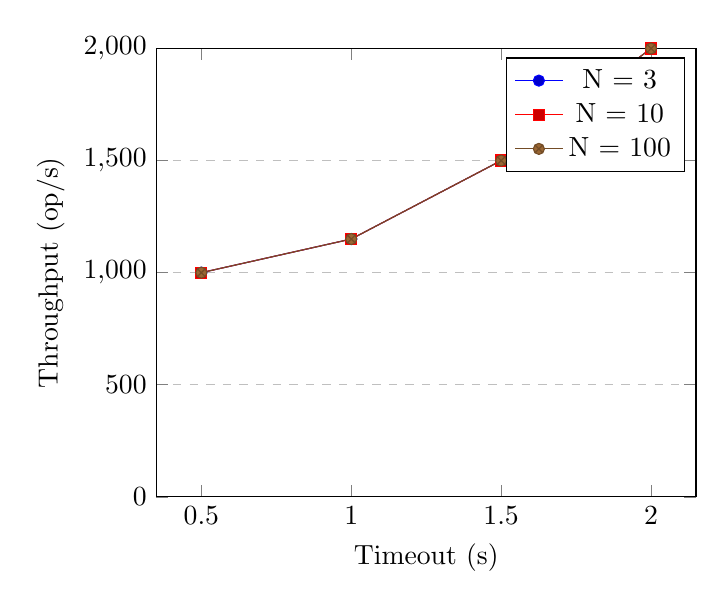
\begin{tikzpicture}
        \begin{axis}[
            xlabel={Timeout (s)},
            ylabel={Throughput (op/s)},
            xtick=data,
            symbolic x coords={0.5, 1, 1.5, 2},
            ymin=0, ymax=2000,
            ymajorgrids=true,
            grid style=dashed
        ]
        \addplot coordinates {(0.5, 1000) (1, 1150) (1.5, 1500) (2, 2000)};
        \addlegendentry{N = 3}
        \addplot coordinates {(0.5, 1000) (1, 1150) (1.5, 1500) (2, 2000)};
        \addlegendentry{N = 10}
        \addplot coordinates {(0.5, 1000) (1, 1150) (1.5, 1500) (2, 2000)};
        \addlegendentry{N = 100}
        \end{axis}
    \end{tikzpicture}
    \caption{Throughput comparison }
\end{subfigure}%
\begin{subfigure}{.55\textwidth}
    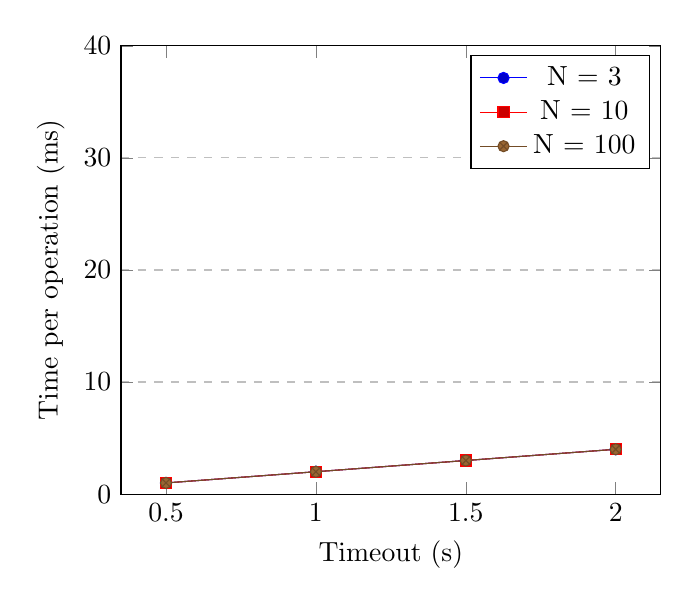
\begin{tikzpicture}
        \begin{axis}[
            xlabel={Timeout (s)},
            ylabel={Time per operation (ms)},
            xtick=data,
            symbolic x coords={0.5, 1, 1.5, 2},
            ymin=0, ymax=40,
            ymajorgrids=true,
            grid style=dashed
        ]
        \addplot coordinates {(0.5, 1) (1, 2) (1.5, 3) (2, 4)};
        \addlegendentry{N = 3}

        \addplot coordinates {(0.5, 1) (1, 2) (1.5, 3) (2, 4)};
        \addlegendentry{N = 10}

        \addplot coordinates {(0.5, 1) (1, 2) (1.5, 3) (2, 4)};
        \addlegendentry{N = 100}
        \end{axis}
    \end{tikzpicture}
    \caption{Operation execution time comparison}
\end{subfigure}
\caption{Performance analysis for a fix number of processes}
\end{figure}

\begin{figure}[ht!]
    \centering
    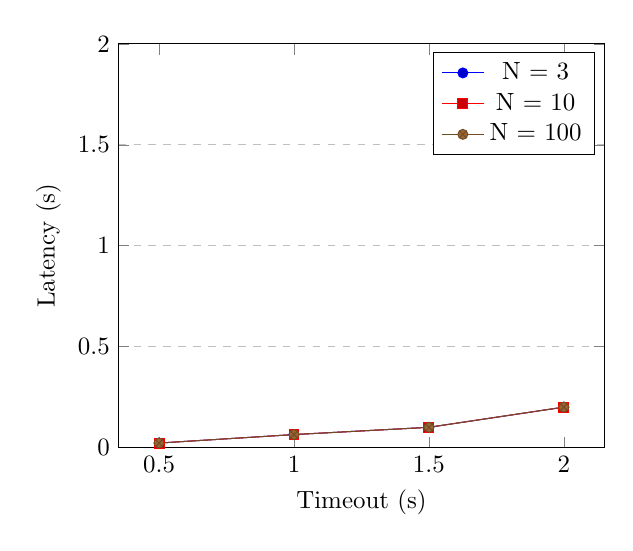
\begin{tikzpicture}[scale=0.9]
        \begin{axis}[
            xlabel={Timeout (s)},
            ylabel={Latency (s)},
            xtick=data,
            symbolic x coords={0.5, 1, 1.5, 2},
            ymin=0, ymax=2,
            ymajorgrids=true,
            grid style=dashed,
        ]
        \addplot coordinates {(0.5, 0.022) (1, 0.064) (1.5, 0.1) (2, 0.2)};
        \addlegendentry{N = 3}

        \addplot coordinates {(0.5, 0.022) (1, 0.064) (1.5, 0.1) (2, 0.2)};
        \addlegendentry{N = 10}

        \addplot coordinates {(0.5, 0.022) (1, 0.064) (1.5, 0.1) (2, 0.2)};
        \addlegendentry{N = 100}
        \end{axis}
    \end{tikzpicture}
    \caption{Latency comparison for a fix number of processes}
\end{figure}

% We can observe that throughput increases with the number of operations
% per process, while the time taken to complete an operation remains almost constant.

% Although we cannot compute many operations in parallel, the throughput
% remains high because the quorum is reached almost instantaneously.

\newpage

\subsection{Results for the probability of failure}
Let's now analyze the results for fix numbers of processes $N$ and timeout $t_{le}$, with different probabilities of failure $\alpha$.

\subsubsection{Results for \(N = 3\) and \(f = 1\)}

\begin{figure}[h!]
    \centering
    \begin{subfigure}{0.55\textwidth}
    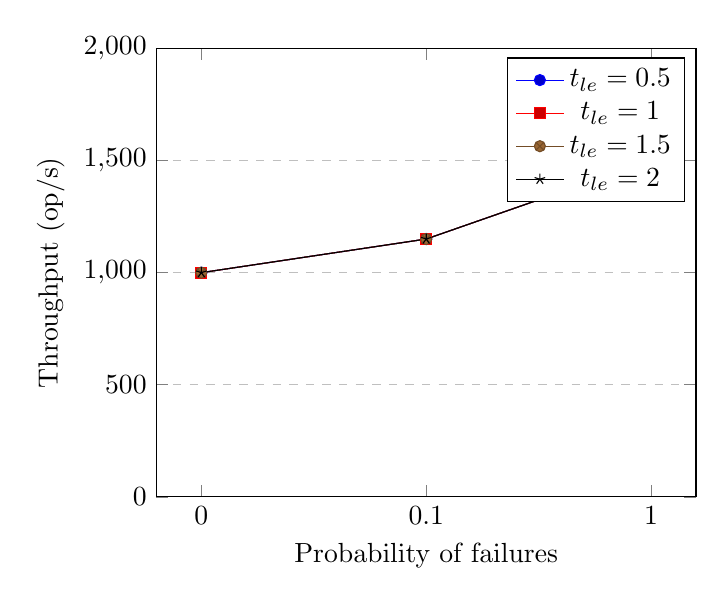
\begin{tikzpicture}
        \begin{axis}[
            xlabel={Probability of failures},
            ylabel={Throughput (op/s)},
            xtick=data,
            symbolic x coords={0, 0.1, 1},
            ymin=0, ymax=2000,
            ymajorgrids=true,
            grid style=dashed
        ]
        \addplot coordinates {(0, 1000) (0.1, 1150) (1, 1500)};
        \addlegendentry{$t_{le} = 0.5$}
        \addplot coordinates {(0, 1000) (0.1, 1150) (1, 1500)};
        \addlegendentry{$t_{le} = 1$}
        \addplot coordinates {(0, 1000) (0.1, 1150) (1, 1500)};
        \addlegendentry{$t_{le} = 1.5$}
        \addplot coordinates {(0, 1000) (0.1, 1150) (1, 1500)};
        \addlegendentry{$t_{le} = 2$}
        \end{axis}
    \end{tikzpicture}
    \caption{Throughput comparison }
\end{subfigure}%
\begin{subfigure}{.55\textwidth}
    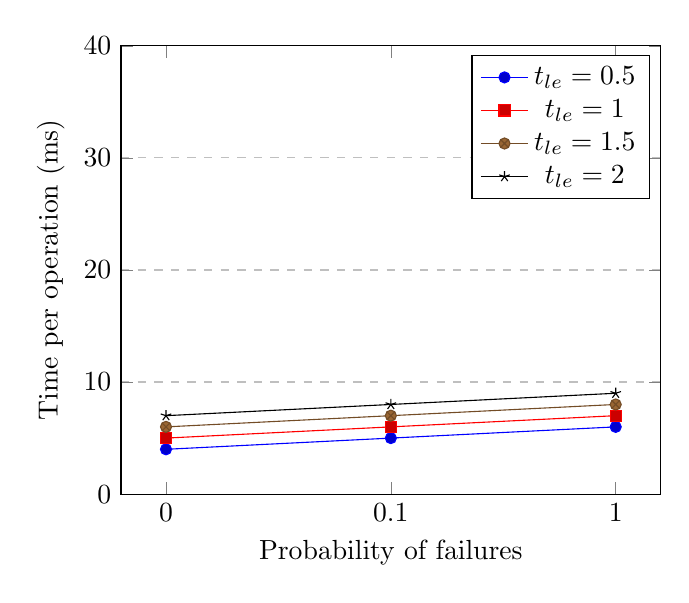
\begin{tikzpicture}
        \begin{axis}[
            xlabel={Probability of failures},
            ylabel={Time per operation (ms)},
            xtick=data,
            symbolic x coords={0, 0.1, 1},
            ymin=0, ymax=40,
            ymajorgrids=true,
            grid style=dashed
        ]
        \addplot coordinates {(0, 4) (0.1, 5) (1, 6)};
        \addlegendentry{$t_{le} = 0.5$}

        \addplot coordinates {(0, 5) (0.1, 6) (1, 7)};
        \addlegendentry{$t_{le} = 1$}
        \addplot coordinates {(0, 6) (0.1, 7) (1, 8)};
        \addlegendentry{$t_{le} = 1.5$}
        \addplot coordinates {(0, 7) (0.1, 8) (1, 9)};
        \addlegendentry{$t_{le} = 2$}
        \end{axis}
    \end{tikzpicture}
    \caption{Operation execution time comparison}
\end{subfigure}
\caption{Performance analysis for \( N = 3 \)}
\end{figure}

\begin{figure}[ht!]
    \centering
    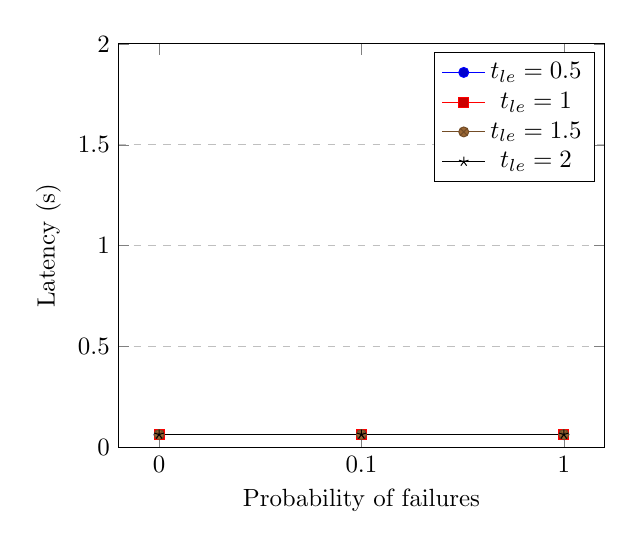
\begin{tikzpicture}[scale=0.9]
        \begin{axis}[
            xlabel={Probability of failures},
            ylabel={Latency (s)},
            xtick=data,
            symbolic x coords={0, 0.1, 1},
            ymin=0, ymax=2,
            ymajorgrids=true,
            grid style=dashed,
        ]
        \addplot coordinates {(0, 0.064) (0.1, 0.064) (1, 0.064)};
        \addlegendentry{$t_{le} = 0.5$}
        \addplot coordinates {(0, 0.064) (0.1, 0.064) (1, 0.064)};
        \addlegendentry{$t_{le} = 1$}
        \addplot coordinates {(0, 0.064) (0.1, 0.064) (1, 0.064)};
        \addlegendentry{$t_{le} = 1.5$}
        \addplot coordinates {(0, 0.064) (0.1, 0.064) (1, 0.064)};
        \addlegendentry{$t_{le} = 2$}
        \end{axis}
    \end{tikzpicture}
    \caption{Latency comparison for \( N = 3 \)}
\end{figure}

\newpage

\subsubsection{Results for \(N = 10\) and \(f = 4\)}

\begin{figure}[h!]
    \centering
    \begin{subfigure}{0.55\textwidth}
    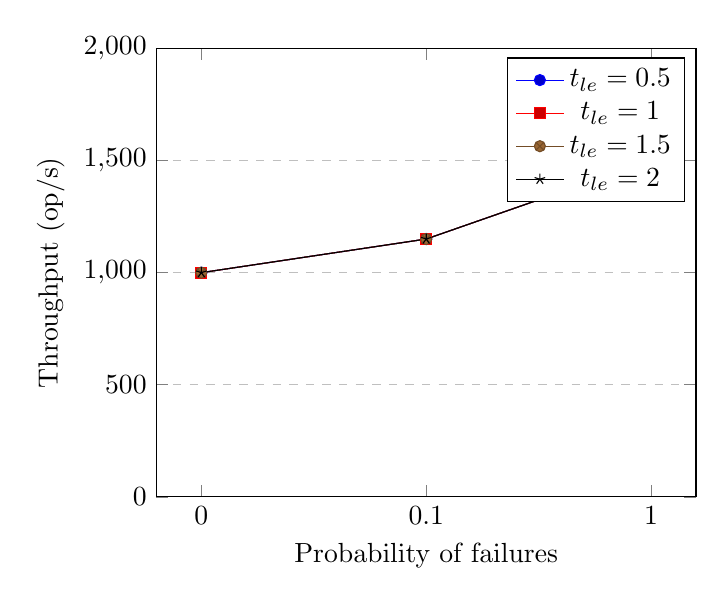
\begin{tikzpicture}
        \begin{axis}[
            xlabel={Probability of failures},
            ylabel={Throughput (op/s)},
            xtick=data,
            symbolic x coords={0, 0.1, 1},
            ymin=0, ymax=2000,
            ymajorgrids=true,
            grid style=dashed
        ]
        \addplot coordinates {(0, 1000) (0.1, 1150) (1, 1500)};
        \addlegendentry{$t_{le} = 0.5$}
        \addplot coordinates {(0, 1000) (0.1, 1150) (1, 1500)};
        \addlegendentry{$t_{le} = 1$}
        \addplot coordinates {(0, 1000) (0.1, 1150) (1, 1500)};
        \addlegendentry{$t_{le} = 1.5$}
        \addplot coordinates {(0, 1000) (0.1, 1150) (1, 1500)};
        \addlegendentry{$t_{le} = 2$}
        \end{axis}
    \end{tikzpicture}
    \caption{Throughput comparison }
\end{subfigure}%
\begin{subfigure}{.55\textwidth}
    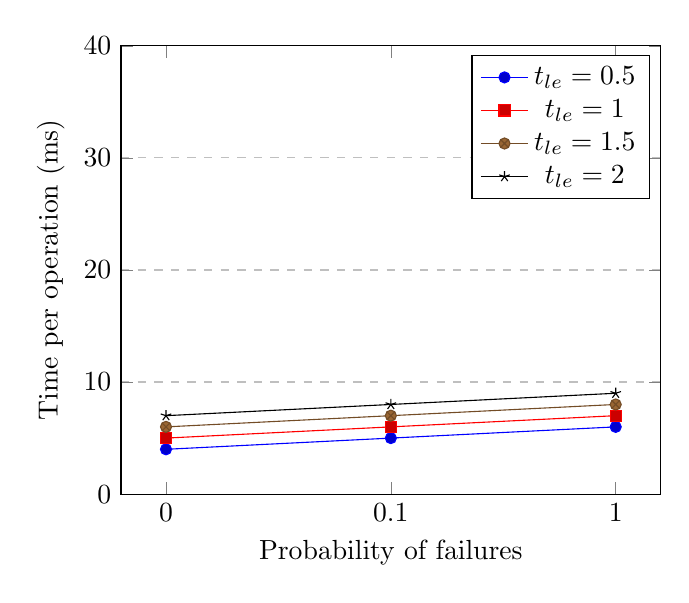
\begin{tikzpicture}
        \begin{axis}[
            xlabel={Probability of failures},
            ylabel={Time per operation (ms)},
            xtick=data,
            symbolic x coords={0, 0.1, 1},
            ymin=0, ymax=40,
            ymajorgrids=true,
            grid style=dashed
        ]
        \addplot coordinates {(0, 4) (0.1, 5) (1, 6)};
        \addlegendentry{$t_{le} = 0.5$}

        \addplot coordinates {(0, 5) (0.1, 6) (1, 7)};
        \addlegendentry{$t_{le} = 1$}
        \addplot coordinates {(0, 6) (0.1, 7) (1, 8)};
        \addlegendentry{$t_{le} = 1.5$}
        \addplot coordinates {(0, 7) (0.1, 8) (1, 9)};
        \addlegendentry{$t_{le} = 2$}
        \end{axis}
    \end{tikzpicture}
    \caption{Operation execution time comparison}
\end{subfigure}
\caption{Performance analysis for \( N = 10 \)}
\end{figure}

\begin{figure}[ht!]
    \centering
    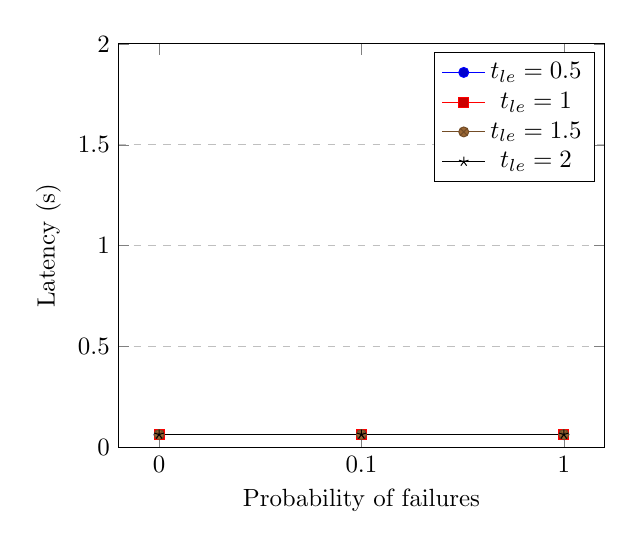
\begin{tikzpicture}[scale=0.9]
        \begin{axis}[
            xlabel={Probability of failures},
            ylabel={Latency (s)},
            xtick=data,
            symbolic x coords={0, 0.1, 1},
            ymin=0, ymax=2,
            ymajorgrids=true,
            grid style=dashed,
        ]
        \addplot coordinates {(0, 0.064) (0.1, 0.064) (1, 0.064)};
        \addlegendentry{$t_{le} = 0.5$}
        \addplot coordinates {(0, 0.064) (0.1, 0.064) (1, 0.064)};
        \addlegendentry{$t_{le} = 1$}
        \addplot coordinates {(0, 0.064) (0.1, 0.064) (1, 0.064)};
        \addlegendentry{$t_{le} = 1.5$}
        \addplot coordinates {(0, 0.064) (0.1, 0.064) (1, 0.064)};
        \addlegendentry{$t_{le} = 2$}
        \end{axis}
    \end{tikzpicture}
    \caption{Latency comparison for \( N = 10 \)}
\end{figure}

\newpage

\subsubsection{Results for \(N = 100\) and \(f = 49\)}

\begin{figure}[h!]
    \centering
    \begin{subfigure}{0.55\textwidth}
    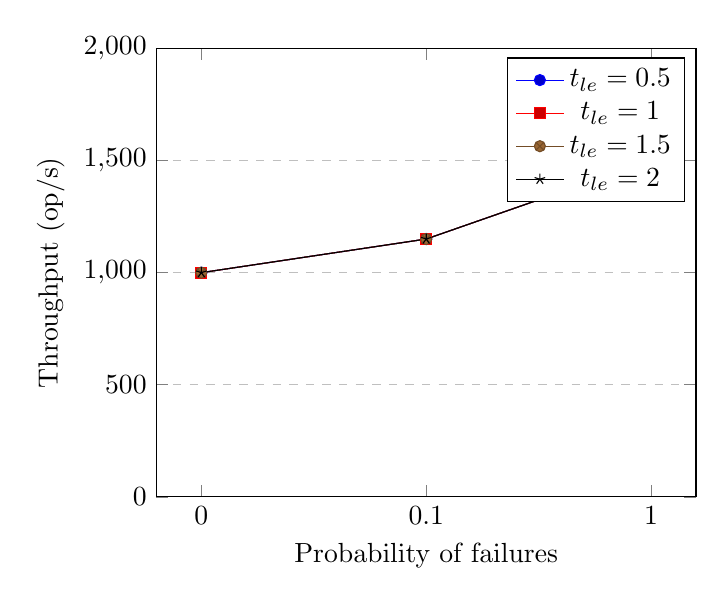
\begin{tikzpicture}
        \begin{axis}[
            xlabel={Probability of failures},
            ylabel={Throughput (op/s)},
            xtick=data,
            symbolic x coords={0, 0.1, 1},
            ymin=0, ymax=2000,
            ymajorgrids=true,
            grid style=dashed
        ]
        \addplot coordinates {(0, 1000) (0.1, 1150) (1, 1500)};
        \addlegendentry{$t_{le} = 0.5$}
        \addplot coordinates {(0, 1000) (0.1, 1150) (1, 1500)};
        \addlegendentry{$t_{le} = 1$}
        \addplot coordinates {(0, 1000) (0.1, 1150) (1, 1500)};
        \addlegendentry{$t_{le} = 1.5$}
        \addplot coordinates {(0, 1000) (0.1, 1150) (1, 1500)};
        \addlegendentry{$t_{le} = 2$}
        \end{axis}
    \end{tikzpicture}
    \caption{Throughput comparison }
\end{subfigure}%
\begin{subfigure}{.55\textwidth}
    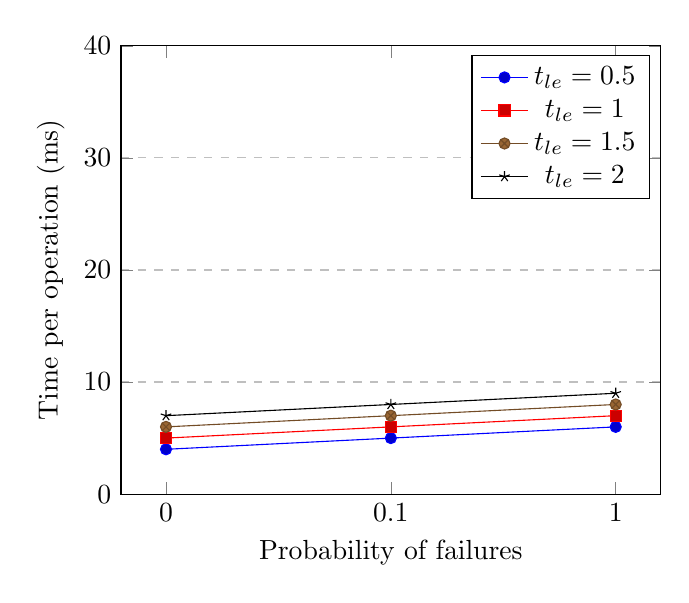
\begin{tikzpicture}
        \begin{axis}[
            xlabel={Probability of failures},
            ylabel={Time per operation (ms)},
            xtick=data,
            symbolic x coords={0, 0.1, 1},
            ymin=0, ymax=40,
            ymajorgrids=true,
            grid style=dashed
        ]
        \addplot coordinates {(0, 4) (0.1, 5) (1, 6)};
        \addlegendentry{$t_{le} = 0.5$}

        \addplot coordinates {(0, 5) (0.1, 6) (1, 7)};
        \addlegendentry{$t_{le} = 1$}
        \addplot coordinates {(0, 6) (0.1, 7) (1, 8)};
        \addlegendentry{$t_{le} = 1.5$}
        \addplot coordinates {(0, 7) (0.1, 8) (1, 9)};
        \addlegendentry{$t_{le} = 2$}
        \end{axis}
    \end{tikzpicture}
    \caption{Operation execution time comparison}
\end{subfigure}
\caption{Performance analysis for \( N = 100 \)}
\end{figure}

\begin{figure}[ht!]
    \centering
    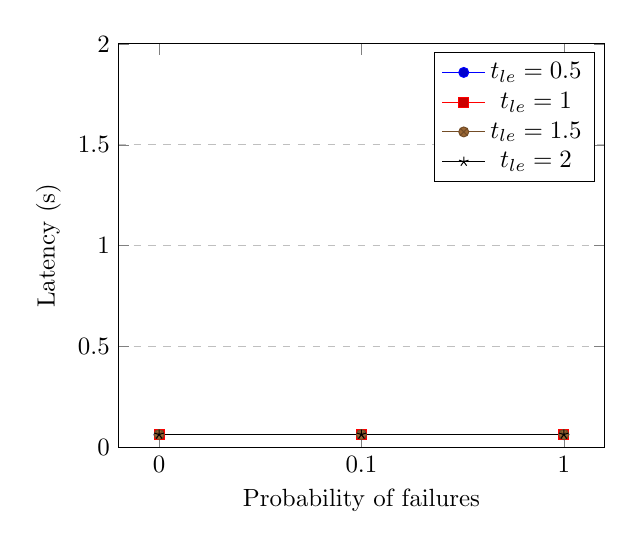
\begin{tikzpicture}[scale=0.9]
        \begin{axis}[
            xlabel={Probability of failures},
            ylabel={Latency (s)},
            xtick=data,
            symbolic x coords={0, 0.1, 1},
            ymin=0, ymax=2,
            ymajorgrids=true,
            grid style=dashed,
        ]
        \addplot coordinates {(0, 0.064) (0.1, 0.064) (1, 0.064)};
        \addlegendentry{$t_{le} = 0.5$}
        \addplot coordinates {(0, 0.064) (0.1, 0.064) (1, 0.064)};
        \addlegendentry{$t_{le} = 1$}
        \addplot coordinates {(0, 0.064) (0.1, 0.064) (1, 0.064)};
        \addlegendentry{$t_{le} = 1.5$}
        \addplot coordinates {(0, 0.064) (0.1, 0.064) (1, 0.064)};
        \addlegendentry{$t_{le} = 2$}
        \end{axis}
    \end{tikzpicture}
    \caption{Latency comparison for \( N = 100 \)}
\end{figure}

\section{Conclusion}
% In conclusion, we can say that the configuration with 3 processes is more
% efficient for a small number of operations, while the configuration with 100
% processes is more efficient for a large number of operations. The configuration
% with 10 processes lies in between.

% If we were to implement this system in a real-life scenario, we would need to
% consider the number of operations to be processed and the acceptable latency.
% Server characteristics and network capacity may also impose constraints that
% influence the choice of the optimal configuration. The configuration with 10
% processes could be a good compromise between the other two in many situations,
% as it is sufficiently efficient for handling both small and large numbers of requests.
\end{document}

